\documentclass[a4paper,11pt]{ltjsarticle}
\usepackage[margin=25mm]{geometry}
\usepackage{luatexja-fontspec}
\setmainfont{DejaVu Serif}
\setsansfont{DejaVu Sans}
\setmainjfont{Noto Serif CJK JP}
\setsansjfont{Noto Sans CJK JP}

\usepackage{amsmath,booktabs,graphicx}
\usepackage[hidelinks,pdfusetitle]{hyperref}


\title{同期固定カメラ映像からのテニスシーン3D再構成}
\author{}
\date{}

\begin{document}
\maketitle

\begin{abstract}
% 全文が揃った段階で要旨を記入する。
\end{abstract}

\section{はじめに}
\label{sec:introduction}

テニス映像から選手の移動と打球の関係を分析するには、関節の運動、コート内での移動、ボールの位置を共通の時刻と座標で表す。
画像上の距離はカメラの向きと撮影距離に依存する。複数視点から奥行きを推定する際も、
白線の見切れ、選手の重なり、球の画面外移動で観測が途切れる。
クリップごとの修正は、復元を支えた観測の追跡と、多数のラリーへの同じ手順の適用を難しくする。

本報告は、同期済み固定カメラ映像を入力とする標準再構成を、幾何推定と実行システムの両面から記述する。
第\ref{sec:problem-and-output}章と第\ref{sec:reconstruction}章で、欠測を含む出力形式と再構成手順を示す。
第\ref{sec:court-detection}章から第\ref{sec:ball-detection}章では、合成教師、選手選別、球像と時間窓を比較し、
観測が失われる過程を調べる。第\ref{sec:execution-system}章と第\ref{sec:experiments}章で、実行システムと実映像での評価を報告する。

\section{関連研究}
\label{sec:related-work}

\section{問題設定と出力形式}
\label{sec:problem-and-output}

\section{再構成手法の全体}
\label{sec:reconstruction}

\section{コート検出}
\label{sec:court-detection}

\section{プレイヤーの3D空間上での追跡}
\label{sec:player-tracking}

\subsection{カメラ内の追跡方式と被覆}

カメラごとに、位置予測と外観の再識別（ReID）で人物検出をローカルIDにまとめる。
StrongSORT++の拡張では、オンラインの外観・運動照合と残余候補のIoU照合にposeコストを加える。
オフラインのAFLinkは、実観測マスクで選んだフレーム番号とboxの左上座標の列から断片を連結する。
GSIの補間は実観測と区別し、保存済みの検出行と実観測マスクを後段に渡す。

Meiji 3camの開発\ev{track-2d}{4}クリップで、保存検出を固定して追跡器を比較した（表\ref{tab:track-2d}）。
StrongSORT++の比較ではAFLinkとGSIの実装・設定・重みを共通とし、オンラインのposeコストを加えると
カメラ内のraw IDF1は\ev{track-2d}{0.930→0.955}に上がった。
Deep OC-SORT＋pose／CLIP＋AFLink／GSIは、このStrongSORT++条件に比べてraw IDF1が低く、pair F1が高かった。
同じStrongSORT++＋poseで高IoUの重複boxを統合すると、\ev{track-merge}{40,531}検出から
\ev{track-merge}{26}件が減り、raw／group IDF1とpair F1は同値だった。

\begin{table}[tbp]
\centering
\caption{保存検出を使った追跡比較。raw IDF1はカメラ内IDのF1、pair F1は視点間の同一人物ペアのF1。
照合は参照boxに対応した件数で、採点可能なペアの被覆も方式によって変わる。}
\label{tab:track-2d}
\small
% Generated by scripts/make_tables.py.
\begin{tabular}{@{}lrrrr@{}}
\toprule
追跡方式 & raw IDF1 & group IDF1 & pair F1 & 照合box \\
\midrule
StrongSORT++ & \ev{track-2d}{0.930} & \ev{track-2d}{0.937} & \ev{track-2d}{0.949} & \ev{track-2d}{25,057/25,147} \\
StrongSORT++＋pose & \ev{track-2d}{0.955} & \ev{track-2d}{0.970} & \ev{track-2d}{0.957} & \ev{track-2d}{25,055/25,147} \\
\shortstack[l]{Deep OC-SORT＋pose／CLIP\\＋AFLink／GSI} & \ev{track-2d}{0.924} & \ev{track-2d}{0.920} & \ev{track-2d}{0.968} & \ev{track-2d}{24,799/25,147} \\
\bottomrule
\end{tabular}

\end{table}

\subsection{コート平面を使う選手選別}

追跡したboxの下辺中央を足元の代理とし、初期校正でコート平面に逆投影する。
コート内外の滞在から選手らしい候補を絞り、足元の連続性とCLIP外観特徴を使ってトラックの断片をつなぐ。
選別した断片の実観測はコート領域外の時刻も保持する。
視点間対応は混合整数線形計画（MILP）で、足元距離と外観の類似度、視点内の排他性と対応の推移性を両立させる。
最良候補の支持や次点との差が足りなければ理由を保存して停止する。

同じDINO・追跡・ViTPose・CLIPの保存出力を用い、選別規則だけを入れ替えた（表\ref{tab:selection-3cam}と表\ref{tab:selection-4cam}）。
予約未見のMeiji 3camでは、観測率・画面中心・boxの高さによる画像上の順位付けを、コート内滞在と断片連結に換えると、
既知の選手boxに対する選別適合率が\ev{selection-3cam}{63.25→100.00\%}、group IDF1が\ev{selection-3cam}{74.98→99.71\%}となった。
raw IDのまま滞在で順位付けしても適合率は上がり、断片連結によって分割された選手のgroup IDF1がさらに上がった。
予約全体のpair F1向上には対応可能になったクリップも寄与した。両方式とも対応が成立した\ev{selection-3cam}{2}本のpair F1は
\ev{selection-3cam}{99.42→99.30\%}だった。4camでは、画像上の順位付けが
\ev{selection-4cam}{0件}、コート滞在と断片連結が\ev{selection-4cam}{55/69件}を三角測量まで進めた。

\begin{table}[tbp]
\centering
\caption{Meiji 3camの選手選別。開発\ev{selection-3cam}{4}本と予約未見\ev{selection-3cam}{3}本の部分参照を採点。
選手P・Rの単位は既知box、group IDF1の単位は参照人物・視点・フレーム。
滞在条件は実験時点のシングルス幅。}
\label{tab:selection-3cam}
\small
% Generated by scripts/make_tables.py.
\begin{tabular}{@{}llrrrrr@{}}
\toprule
集合 & 選別 & 選手P [\%] & 選手R [\%] & group IDF1 [\%] & pair F1 [\%] & 成立 \\
\midrule
開発 & 画像上の順位付け & \ev{selection-3cam}{85.55} & \ev{selection-3cam}{95.37} & \ev{selection-3cam}{88.46} & \ev{selection-3cam}{63.56} & \ev{selection-3cam}{2/4} \\
開発 & コート滞在（raw ID） & \ev{selection-3cam}{99.66} & \ev{selection-3cam}{94.31} & \ev{selection-3cam}{96.14} & \ev{selection-3cam}{94.13} & \ev{selection-3cam}{4/4} \\
開発 & コート滞在＋連結 & \ev{selection-3cam}{99.98} & \ev{selection-3cam}{95.32} & \ev{selection-3cam}{96.99} & \ev{selection-3cam}{95.71} & \ev{selection-3cam}{4/4} \\
予約 & 画像上の順位付け & \ev{selection-3cam}{63.25} & \ev{selection-3cam}{99.17} & \ev{selection-3cam}{74.98} & \ev{selection-3cam}{77.35} & \ev{selection-3cam}{2/3} \\
予約 & コート滞在（raw ID） & \ev{selection-3cam}{100.00} & \ev{selection-3cam}{99.17} & \ev{selection-3cam}{96.69} & \ev{selection-3cam}{99.24} & \ev{selection-3cam}{3/3} \\
予約 & コート滞在＋連結 & \ev{selection-3cam}{100.00} & \ev{selection-3cam}{99.29} & \ev{selection-3cam}{99.71} & \ev{selection-3cam}{99.43} & \ev{selection-3cam}{3/3} \\
\bottomrule
\end{tabular}

\end{table}

\begin{table}[tbp]
\centering
\caption{Meiji 4camの選別と三角測量の成立。コートの向きは選手観測で判定した。
完了は有効な人物関節を持つクリップ。
被覆の分母は全\ev{selection-4cam}{69}件の\ev{selection-4cam}{184,912}選手フレーム。}
\label{tab:selection-4cam}
\small
% Generated by scripts/make_tables.py.
\begin{tabular}{@{}lrrr@{}}
\toprule
選別 & 三角測量完了 & 有効選手フレーム & 被覆率 [\%] \\
\midrule
選別なし & \ev{selection-4cam}{0/69} & \ev{selection-4cam}{0} & \ev{selection-4cam}{0.00} \\
画像上の順位付け & \ev{selection-4cam}{0/69} & \ev{selection-4cam}{0} & \ev{selection-4cam}{0.00} \\
コート滞在（raw ID） & \ev{selection-4cam}{52/69} & \ev{selection-4cam}{126,952} & \ev{selection-4cam}{68.66} \\
コート滞在＋連結 & \ev{selection-4cam}{55/69} & \ev{selection-4cam}{133,887} & \ev{selection-4cam}{72.41} \\
\bottomrule
\end{tabular}

\end{table}

\subsection{停止時に失われた2D観測}

実映像で停止した\ev{stopped}{14}クリップでは、同じ元フレームの全視点で、DINOのbox、追跡ID、選別グループ、対応結果を照合した。
基本\ev{stopped}{42}時点で評価可能な\ev{stopped}{665}選手・視点枠すべてに人物boxと追跡IDがあり、選別後に残ったのは\ev{stopped}{581}枠だった。
選手の重なりで追跡IDが交代した例を図\ref{fig:stopped-004}に、選別で選手が全視点から外れた例を図\ref{fig:stopped-020}に示す。
選手候補の境界で停止した\ev{stopped}{9}件すべてで次点グループに実選手が含まれ、同一選手が視点によって別の対応IDに分かれていた。

\begin{figure}[tbp]
\centering
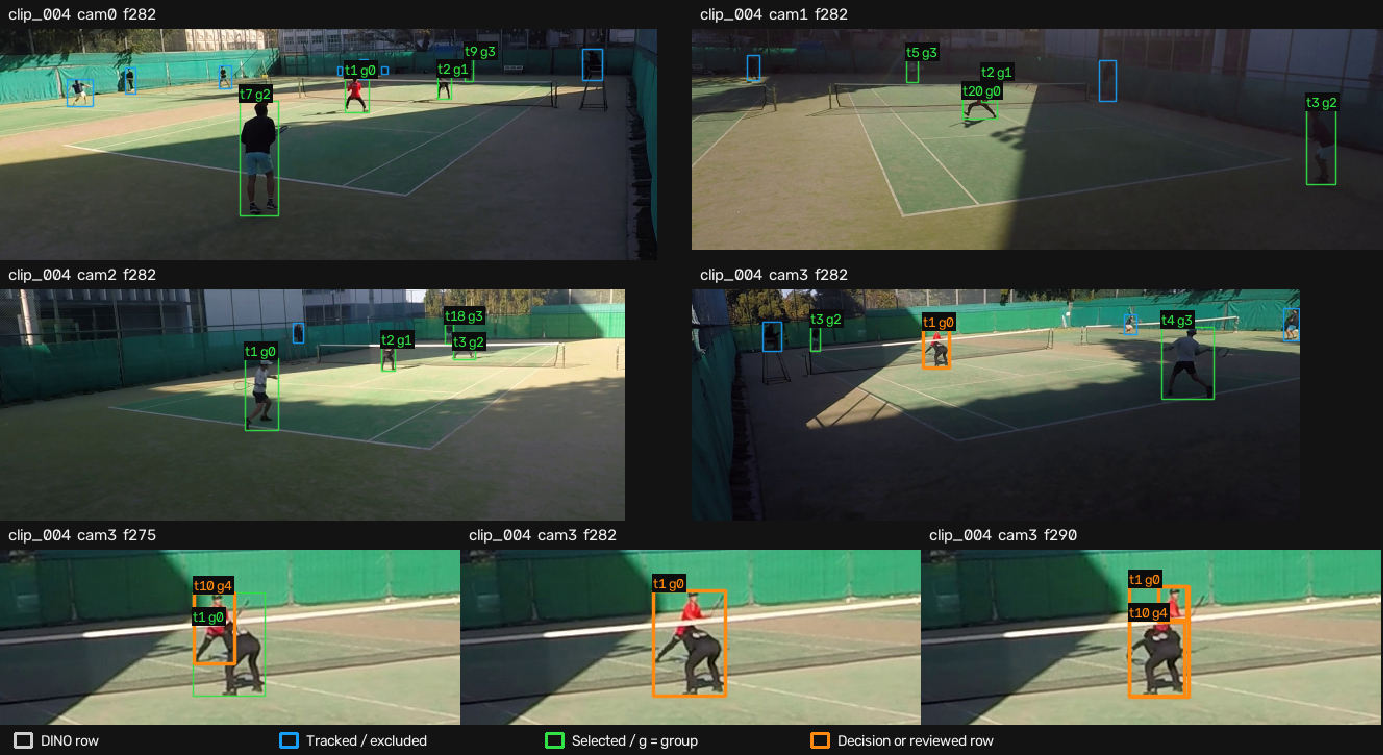
\includegraphics[width=\linewidth]{figures/players/clip_004-f0282.pdf}
\caption{clip\_004の元フレーム\ev{stopped-scenes}{282}の同期\ev{stopped-scenes}{4}視点と、cam3の前後。
cam3で重なった選手を同じboxが囲み、前後で追跡IDが交代した。
橙は診断対象、緑は選別済み、青は追跡済み・選別外、灰は追跡IDのない検出。}
\label{fig:stopped-004}
\end{figure}

\begin{figure}[tbp]
\centering
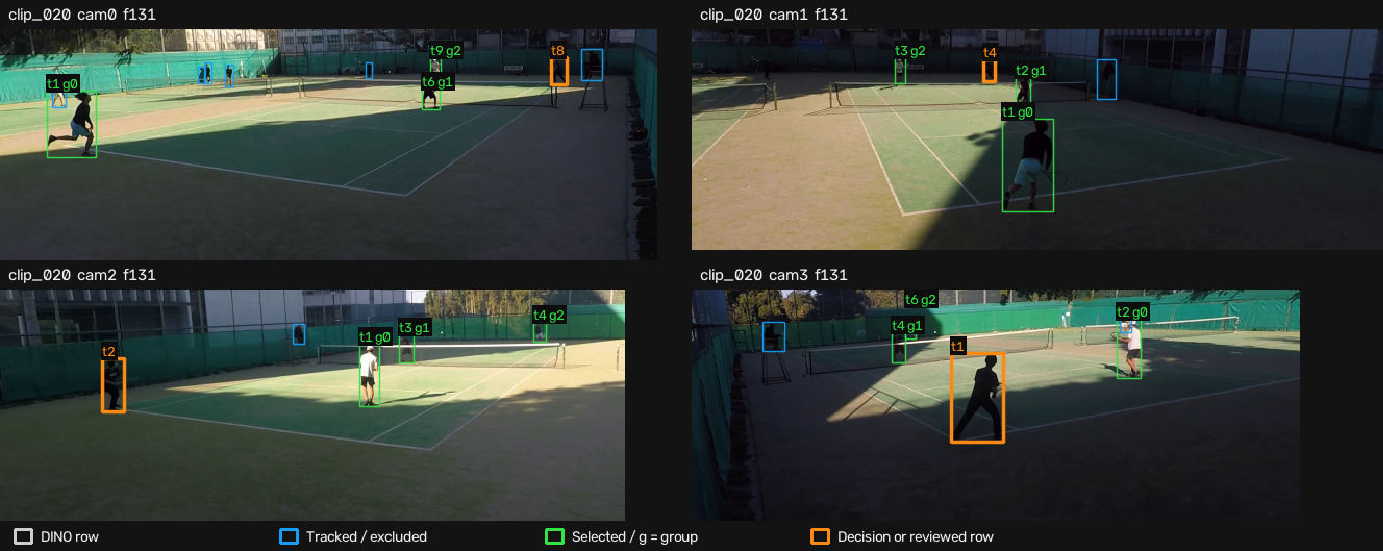
\includegraphics[width=\linewidth]{figures/players/clip_020-f0131.pdf}
\caption{clip\_020の元フレーム\ev{stopped-scenes}{131}の同期\ev{stopped-scenes}{4}視点。
不足した選手のboxとローカルIDが各視点に存在し、選別から外れていた。色は図\ref{fig:stopped-004}と同じ。}
\label{fig:stopped-020}
\end{figure}

保存特徴での再生は元の停止コードを\ev{stopped-replay}{14/14}件で再現した。
目視で確かめたDINO行の除去では\ev{stopped-replay}{0/8}件、同一選手と判断したグループの統合では\ev{stopped-replay}{0/2}件が回復した。
次点グループだけを外す感度比較では\ev{stopped-replay}{7/9}件が人物対応を通過し、
そのうち\ev{stopped-replay}{5}件で、レビューした時点の全選手が各\ev{stopped-replay}{2}視点以上に同じIDで残った。

\subsection{3Dで時間IDを決める選択経路}

現行の選択経路 \texttt{multiview\_3d\_tracking} は、全人物の2D関節から各時刻の3D骨格候補を作り、観測を排他的に割り当てる。
重なりや欠測をまたぐ時間窓で3D候補を結び、コート上の軌跡から選手を選別する。
複数視点の観測でカメラ内の途切れを補い、選手IDと対応する元検出行を身体復元へ渡す。

\begin{table}[tbp]
\centering
\caption{旧経路と3D時間追跡の比較。計測版は統合前の開発ブランチ。
4camでは同じ幾何と球を使い、全選手の身体復元・配置と球3Dを確認できたクリップを完了とした。
方式ごとに、関節の推定に使わなかった観測を採点し、クリップごとに再投影残差の中央値を求めた。}
\label{tab:tracking-3d}
\small
% Generated by scripts/make_tables.py.
\begin{tabular}{@{}lrr@{}}
\toprule
測定項目 & 旧経路 & 3D時間追跡 \\
\midrule
4cam 完了クリップ & \ev{track-3d-4cam}{52/69} & \ev{track-3d-4cam}{69/69} \\
4cam 全員の有効配置 [\%] & \ev{track-3d-4cam}{64.63} & \ev{track-3d-4cam}{90.74} \\
4cam 共通\ev{track-3d-4cam}{55}本の再投影中央値 [px] & \ev{track-3d-4cam}{7.89} & \ev{track-3d-4cam}{24.86} \\
3cam 予約未見のIDF1 [\%] & \ev{track-3d-3cam}{92.07} & \ev{track-3d-3cam}{80.42} \\
3cam 予約未見の選別再現率 [\%] & \ev{track-3d-3cam}{85.30} & \ev{track-3d-3cam}{67.25} \\
\bottomrule
\end{tabular}

\end{table}

Meiji 4camで完了は\ev{track-3d-4cam}{52/69→69/69}件に増え、選手再構成の停止は\ev{track-3d-4cam}{14→0}件に減った（表\ref{tab:tracking-3d}）。
予約未見のMeiji 3camでは射影した時間IDのIDF1が\ev{track-3d-3cam}{92.07→80.42\%}に下がった。
旧経路が校正で停止して新経路で補完した\ev{track-3d-3cam}{1}本を除いても、IDF1の低下が残った。
4camの共通クリップでは、再投影残差がクリップ中央値の中央値で\ev{track-3d-4cam}{7.89→24.86} pxへ増えた。

\section{ボール検出}
\label{sec:ball-detection}

\subsection{標準モデルと外部注釈}

標準経路は、i935の時系列検出器でカメラごとに球の位置と存在スコアを推定する。
入力映像から作るMDDは、隣接時刻の変化を符号別に表す差分特徴である。
i935はMDDの\ev{ball-config}{2}チャネルを受け取り、\ev{ball-config}{8}フレームの窓を使う。
同一フレームを複数窓が覆う場合は窓の中心に近い予測を採用し、候補点を運動整合の検査へ渡す。
別設定として、RGBとMDDを入力とするX3D／CSN系の動画エンコーダ\cite{x3d,csn}に
DPT型の高密度デコーダ\cite{dpt}をつないだ\ev{ball-x3d}{32}フレームの球検出器を用意した。
Meiji 4camのclip\_000からcam1〜cam3を使い、X3Dで得たカメラ幾何を両方式に固定して診断した。
有効な球3Dはi935で\ev{ball-x3d}{113/356}、X3Dで\ev{ball-x3d}{123/356}元フレームだった。
校正と向き判定を含む同じ視点の通常実行では、i935はコート向きが決まらず停止した。
固定幾何で球観測を比べた結果と、校正・向き判定を含む処理の成立は別の評価となる。

保存済み注釈を固定の幾何へ渡す経路もある。
Meiji 4camの外部座標初版\ev{ball-origin}{69} JSONは、
Chromeが\ev{ball-origin}{2026年11月24日 01:50:43 UTC}に \texttt{chatgpt.com} から取得した記録のあるZIPと全件バイト一致した。
これは取得経路の来歴であり、初版を生成したモデルと実行IDは保存記録からは確定できなかった。
後続の再注釈は同日\ev{ball-origin}{20:27 JST}にCodex CLIのGPT-6.2 Sol（effort max）で開始し、
clip\_012、clip\_015、clip\_026の出力が公開rev1の対応ファイルと一致した。
初版を以下の球像と可視性の診断に用い、rev1の\ev{ball-origin}{3}本はベンチマークの注釈更新に対応する。

\subsection{球像の大きさ・ブラー・可視性}

Meiji 4camの\ev{ball-footprint}{69}クリップでは元画像が\ev{ball-footprint}{1920×1080}、約\ev{ball-footprint}{59.94} fpsだった。
画面内の観測ラベルからカメラ別・クリップ別に時点を選び、前後画像の中央値で作った背景を引いた。
注釈の周辺にある同符号の残差成分から、短軸分散で円盤相当径を、長短軸の分散差で見かけの伸び（ブラー指標）を求めた。
同じ時点を縮小して測定し、成分の面積やコントラストが足りない場合は欠測とした。
元画像では\ev{ball-footprint}{2,121/2,208}件が測れ、径の中央値は\ev{ball-footprint}{4.00} pxだった。
\ev{ball-footprint}{512×288}では\ev{ball-footprint}{360/2,208}件が測れ、
径の中央値は\ev{ball-footprint}{1.76} pxだった。全サイズで測れた\ev{ball-footprint}{339}件を揃えた比較でも、
縮小に伴って径が小さくなった（図\ref{fig:ball-footprints}）。表\ref{tab:ball-cameras}で視点ごとの差を示す。

\begin{figure}[tbp]
\centering
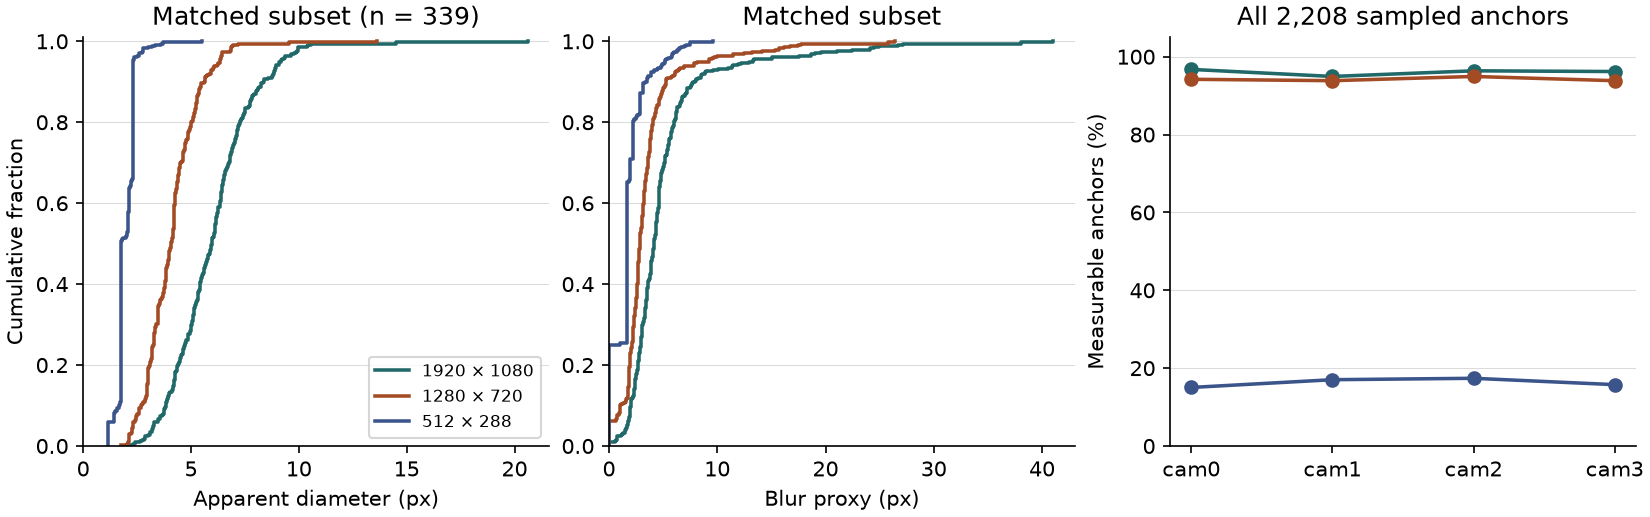
\includegraphics[width=\linewidth]{figures/ball/footprint-distributions.png}
\caption{外部座標付近で測った球像の径と見かけの伸び。左・中央は全サイズで測れた同じ
\ev{ball-footprint}{339}件の累積分布（測定画像px）。右は抽出した\ev{ball-footprint}{2,208}件での視点別の計測成立率。}
\label{fig:ball-footprints}
\end{figure}

\begin{table}[tbp]
\centering
\caption{Meiji 4camの視点別診断。径・伸びは元画像で計測成立した成分の中央値。
範囲外座標は各視点の\ev{ball-visibility}{46,228}座標、可視確認は層化抽出した各視点の\ev{ball-visibility}{16}件を分母とする。}
\label{tab:ball-cameras}
\small
% Generated by scripts/make_tables.py.
\begin{tabular}{@{}lrrrrr@{}}
\toprule
視点 & 計測成立 & 径 [px] & 伸び [px] & 範囲外座標 & 可視確認 \\
\midrule
cam0 & \ev{ball-footprint}{534/552} & \ev{ball-footprint}{3.94} & \ev{ball-footprint}{2.55} & \ev{ball-visibility}{688} & \ev{ball-visibility}{6/16} \\
cam1 & \ev{ball-footprint}{524/552} & \ev{ball-footprint}{3.71} & \ev{ball-footprint}{2.67} & \ev{ball-visibility}{630} & \ev{ball-visibility}{9/16} \\
cam2 & \ev{ball-footprint}{532/552} & \ev{ball-footprint}{4.20} & \ev{ball-footprint}{2.90} & \ev{ball-visibility}{756} & \ev{ball-visibility}{6/16} \\
cam3 & \ev{ball-footprint}{531/552} & \ev{ball-footprint}{4.19} & \ev{ball-footprint}{2.42} & \ev{ball-visibility}{2,062} & \ev{ball-visibility}{6/16} \\
\bottomrule
\end{tabular}

\end{table}

初版の視点・フレーム別外部座標で、画像境界の外に中心があるのは
\ev{ball-visibility}{4,136/184,912}件（\ev{ball-visibility}{2.24\%}）だった。
うち\ev{ball-visibility}{4,125}件には推定座標の区分が付いていた。
画像内の観測、その他の画像内、範囲外座標から層化した目視監査では、
\ev{ball-visibility}{64}件のうち可視\ev{ball-visibility}{27}件、遮蔽\ev{ball-visibility}{2}件、
画面内で識別不能\ev{ball-visibility}{11}件、退出を視認した画面外\ev{ball-visibility}{1}件だった。
範囲外座標の\ev{ball-visibility}{16}件中\ev{ball-visibility}{15}件は退出を視認できなかった。
図\ref{fig:ball-visibility}の目視件数は層化した標本に対する値で、座標範囲外の比率とも評価対象が異なる。

\begin{figure}[tbp]
\centering
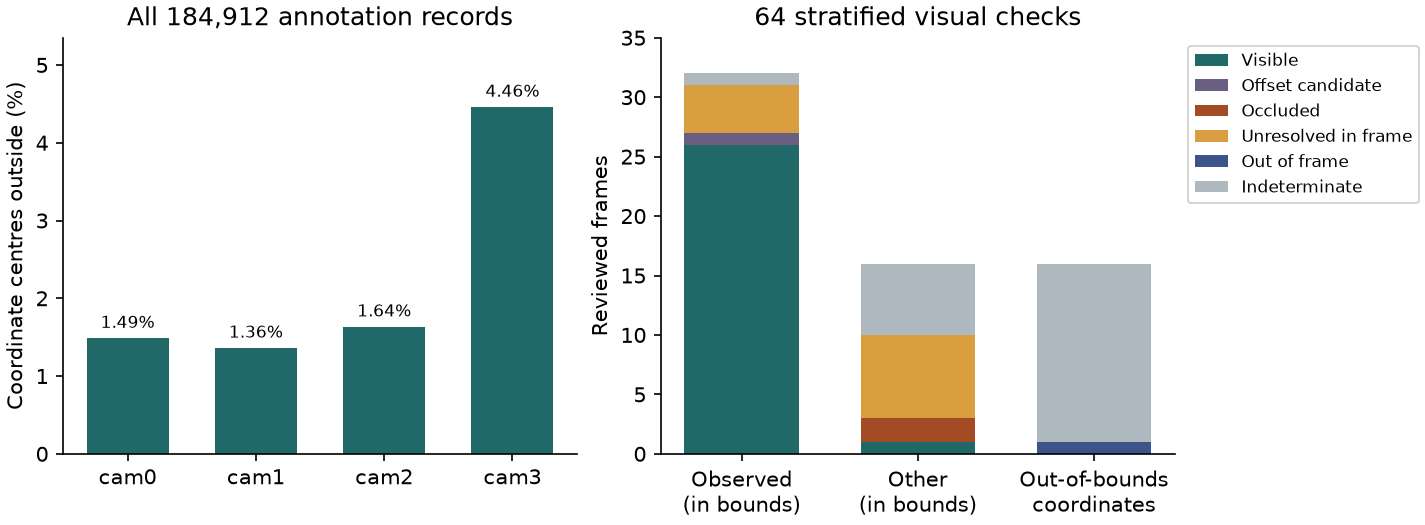
\includegraphics[width=\linewidth]{figures/ball/visibility.png}
\caption{外部座標中心の範囲外率と層化目視監査。座標の全数集計と、映像中で見え方を確認した監査を併記した。}
\label{fig:ball-visibility}
\end{figure}

\subsection{既存の容量・系列長と人工カメラ変動}

球像が縮小で識別しにくくなると、増やしたパラメータがどの程度位置精度に寄与するかは、同じ採点集合で調べる必要がある。
表\ref{tab:ball-history}の容量比較では、共通の長系列validationで最小の約\ev{ball-capacity}{8.0}百万パラメータの条件でも
平均\ev{ball-capacity}{35.38} px、P95 \ev{ball-capacity}{169.69} pxの誤差が残った。
容量を増やした条件で平均は下がったが、誤差分布の裾は大きい。
別の逐次学習のDPT系列では、\ev{ball-length}{32→64}フレームで位置誤差は下がり、更新数は増加した。
また、合成のカメラ変動を加えたConvNeXt＋queryの診断では平均位置誤差が
\ev{ball-camera-stress}{15.4→32.2}元画像pxへ増えた。これは元画像と座標に同じ画像変換を適用し、
変換後の画面外を採点から外した実験であり、撮影機材だけを入れ替えた測定とは条件が異なる。

\begin{table}[tbp]
\centering
\caption{既存の長系列validationでの代表比較。位置の単位は元画像px、採点対象は\ev{ball-length}{85,473}観測フレーム。
逐次学習の行は累積更新数、容量比較の行はquery学習の更新数を示す。}
\label{tab:ball-history}
\small
% Generated by scripts/make_tables.py.
\begin{tabular}{@{}lrrrrr@{}}
\toprule
条件 & 窓長 & 百万parameter & 更新 & 平均 [px] & P95 [px] \\
\midrule
common-dpt-T32 & \ev{ball-length}{32} & \ev{ball-length}{—} & \ev{ball-length}{10,000} & \ev{ball-length}{42.58} & \ev{ball-length}{248.14} \\
dpt-T64 & \ev{ball-length}{64} & \ev{ball-length}{—} & \ev{ball-length}{16,000} & \ev{ball-length}{36.56} & \ev{ball-length}{183.20} \\
query-T32 & \ev{ball-length}{32} & \ev{ball-length}{—} & \ev{ball-length}{16,000} & \ev{ball-length}{42.99} & \ev{ball-length}{136.21} \\
query-T64 & \ev{ball-length}{64} & \ev{ball-length}{—} & \ev{ball-length}{22,000} & \ev{ball-length}{28.20} & \ev{ball-length}{116.89} \\
d256-L4 & \ev{ball-capacity}{64} & \ev{ball-capacity}{8.0} & \ev{ball-capacity}{12,000} & \ev{ball-capacity}{35.38} & \ev{ball-capacity}{169.69} \\
d384-L4 & \ev{ball-capacity}{64} & \ev{ball-capacity}{13.3} & \ev{ball-capacity}{12,000} & \ev{ball-capacity}{35.11} & \ev{ball-capacity}{167.50} \\
d512-L4 & \ev{ball-capacity}{64} & \ev{ball-capacity}{21.0} & \ev{ball-capacity}{12,000} & \ev{ball-capacity}{33.58} & \ev{ball-capacity}{164.14} \\
d768-L4 & \ev{ball-capacity}{64} & \ev{ball-capacity}{41.9} & \ev{ball-capacity}{12,000} & \ev{ball-capacity}{33.88} & \ev{ball-capacity}{160.81} \\
d1024-L4 & \ev{ball-capacity}{64} & \ev{ball-capacity}{71.8} & \ev{ball-capacity}{12,000} & \ev{ball-capacity}{33.38} & \ev{ball-capacity}{161.51} \\
d512-L6 & \ev{ball-capacity}{64} & \ev{ball-capacity}{29.7} & \ev{ball-capacity}{12,000} & \ev{ball-capacity}{34.26} & \ev{ball-capacity}{162.06} \\
d512-L8 & \ev{ball-capacity}{64} & \ev{ball-capacity}{38.3} & \ev{ball-capacity}{12,000} & \ev{ball-capacity}{32.48} & \ev{ball-capacity}{149.47} \\
\bottomrule
\end{tabular}

\end{table}

\subsection{学習済みモデルへの時間文脈の介入}

固定validationから\ev{ball-intervention}{144}アンカーを選び、球を観測した\ev{ball-intervention}{88}件で位置精度を測った。
同じチェックポイント・アンカー・存在閾値で、通常の時系列、アンカー画像の反復、周辺画像をシャッフルする条件を比較した。
RGBからMDDを作る処理は全条件で同じで、アンカーの位置も固定した。
形状ベースの対照では局所コントラスト、丸さ、白・黄の色、背景差分を使い、別収録群で存在閾値を選んだ。

表\ref{tab:ball-intervention}では、位置が\ev{ball-intervention}{20}元画像px以内の件数が、
X3D T32で通常\ev{ball-intervention}{76/88（86.36\%）}から反復\ev{ball-intervention}{2/88（2.27\%）}へ、
i935 T8で通常\ev{ball-intervention}{73/88（82.95\%）}から反復\ev{ball-intervention}{0/88}へ落ちた。
周辺の順序を変えた場合も、全体では両モデルで命中数が減った。形状対照は\ev{ball-intervention}{7/88（7.95\%）}で、
欠測や背景の紛らわしい像も含めたこの集合では、形状と短い背景差分の組合せから球を分けるのが難しかった。

\begin{table}[tbp]
\centering
\caption{固定アンカーに対する推論時の介入。位置は存在閾値を適用する前の予測で採点し、
存在の偽陽性は確認不在\ev{ball-intervention}{56}件、偽陰性は観測\ev{ball-intervention}{88}件を分母とする。
X3Dと形状対照は\ev{ball-intervention}{1280×720}、i935は\ev{ball-intervention}{512×288}。}
\label{tab:ball-intervention}
\small
% Generated by scripts/make_tables.py.
\begin{tabular}{@{}llrrrrr@{}}
\toprule
モデル & 入力 & 平均 [px] & P95 [px] & 命中 & FPR [\%] & FNR [\%] \\
\midrule
X3D T32 & 通常 & \ev{ball-intervention}{24.22} & \ev{ball-intervention}{66.31} & \ev{ball-intervention}{76/88} & \ev{ball-intervention}{21.43} & \ev{ball-intervention}{14.77} \\
X3D T32 & 同一画像を反復 & \ev{ball-intervention}{253.86} & \ev{ball-intervention}{699.98} & \ev{ball-intervention}{2/88} & \ev{ball-intervention}{0.00} & \ev{ball-intervention}{100.00} \\
X3D T32 & 周辺の順序入替え & \ev{ball-intervention}{88.48} & \ev{ball-intervention}{510.17} & \ev{ball-intervention}{55/88} & \ev{ball-intervention}{17.86} & \ev{ball-intervention}{34.09} \\
i935 T8 & 通常 & \ev{ball-intervention}{34.94} & \ev{ball-intervention}{230.85} & \ev{ball-intervention}{73/88} & \ev{ball-intervention}{14.29} & \ev{ball-intervention}{17.05} \\
i935 T8 & 同一画像を反復 & \ev{ball-intervention}{233.16} & \ev{ball-intervention}{494.07} & \ev{ball-intervention}{0/88} & \ev{ball-intervention}{0.00} & \ev{ball-intervention}{100.00} \\
i935 T8 & 周辺の順序入替え & \ev{ball-intervention}{58.01} & \ev{ball-intervention}{302.58} & \ev{ball-intervention}{67/88} & \ev{ball-intervention}{14.29} & \ev{ball-intervention}{36.36} \\
形状対照 & 色・丸さ・背景差分 & \ev{ball-intervention}{458.73} & \ev{ball-intervention}{987.17} & \ev{ball-intervention}{7/88} & \ev{ball-intervention}{62.50} & \ev{ball-intervention}{40.91} \\
\bottomrule
\end{tabular}

\end{table}

\subsection{同一予算での単フレーム学習と時系列学習}

推論時の反復に加え、各入力で最初から学習し直した。同じX3D／CSN＋DPTを
\ev{ball-train-plan}{512×288}、seed \ev{ball-train-plan}{42}、
\ev{ball-train-plan}{30,478}学習パックで比較し、初期重みの共通部分と抽出順を揃えた。
各条件は\ev{ball-train-plan}{4,700}更新、更新当たり\ev{ball-train-plan}{128}枚、計\ev{ball-train-plan}{601,600}入力フレームだった。
単フレームにはRGBを、時系列にはRGBと各窓から計算したMDDを入力した。

全validationの\ev{ball-train-val}{117,358}件（observed \ev{ball-train-val}{85,473}件）では、
\ev{ball-train-val}{20} px以内率が単フレームRGBの\ev{ball-train-val}{1.66\%}から、
\ev{ball-train-plan}{T=8}で\ev{ball-train-val}{40.90\%}、\ev{ball-train-plan}{T=32}で\ev{ball-train-val}{44.23\%}に上がった。
Chat、Meiji 3cam、TrackNet game9のすべてで上がり、同じ\ev{ball-train-anchor}{144}アンカーでも
\ev{ball-train-anchor}{2/88→40/88→45/88}と増えた（表\ref{tab:ball-training}、図\ref{fig:ball-training}）。
存在F1は各条件のvalidationでFPRとFNRの平均が最小となる閾値で集計した。位置採点にはこの閾値を適用しない。

単フレームからの差にはMDDの有無が含まれる。
両方でRGB＋MDDを使う\ev{ball-train-plan}{T=8とT=32}の比較では、
窓の延長に伴う改善は全validationで\ev{ball-train-val}{3.33}ポイント、アンカーで\ev{ball-train-anchor}{5.68}ポイントだった。
単一seed・固定解像度での結果で、独立testは今後の評価に含める。
この学習比較と前節のチェックポイント比較では、学習履歴と入力解像度が異なる。

\begin{table}[tbp]
\centering
\caption{入力条件ごとに学習した検出器の成績。位置誤差はobservedの元画像px。
収録元別の\ev{ball-train-val}{20} px以内率の分母は、Chat \ev{ball-train-sources}{61,369}件、
Meiji 3cam \ev{ball-train-sources}{23,007}件、TrackNet game9 \ev{ball-train-sources}{1,097}件。}
\label{tab:ball-training}
\small
% Generated by scripts/make_tables.py.
\begin{tabular}{@{}lrrr@{}}
\toprule
指標 & \ev{ball-train-plan}{T=1} RGB & \ev{ball-train-plan}{T=8} RGB＋MDD & \ev{ball-train-plan}{T=32} RGB＋MDD \\
\midrule
平均位置誤差 [px] & \ev{ball-train-val}{226.75} & \ev{ball-train-val}{134.06} & \ev{ball-train-val}{125.74} \\
中央値位置誤差 [px] & \ev{ball-train-val}{177.02} & \ev{ball-train-val}{42.48} & \ev{ball-train-val}{31.68} \\
全validationの命中率 [\%] & \ev{ball-train-val}{1.66} & \ev{ball-train-val}{40.90} & \ev{ball-train-val}{44.23} \\
存在F1 [\%] & \ev{ball-train-val}{74.07} & \ev{ball-train-val}{82.02} & \ev{ball-train-val}{82.63} \\
Chatの命中率 [\%] & \ev{ball-train-sources}{1.29} & \ev{ball-train-sources}{45.54} & \ev{ball-train-sources}{49.20} \\
Meiji 3camの命中率 [\%] & \ev{ball-train-sources}{2.66} & \ev{ball-train-sources}{27.36} & \ev{ball-train-sources}{29.77} \\
TrackNet game9の命中率 [\%] & \ev{ball-train-sources}{1.37} & \ev{ball-train-sources}{65.18} & \ev{ball-train-sources}{69.10} \\
固定アンカーの命中数（率 [\%]） & \ev{ball-train-anchor}{2/88（2.27）} & \ev{ball-train-anchor}{40/88（45.45）} & \ev{ball-train-anchor}{45/88（51.14）} \\
\bottomrule
\end{tabular}

\end{table}

\begin{figure}[tbp]
\centering
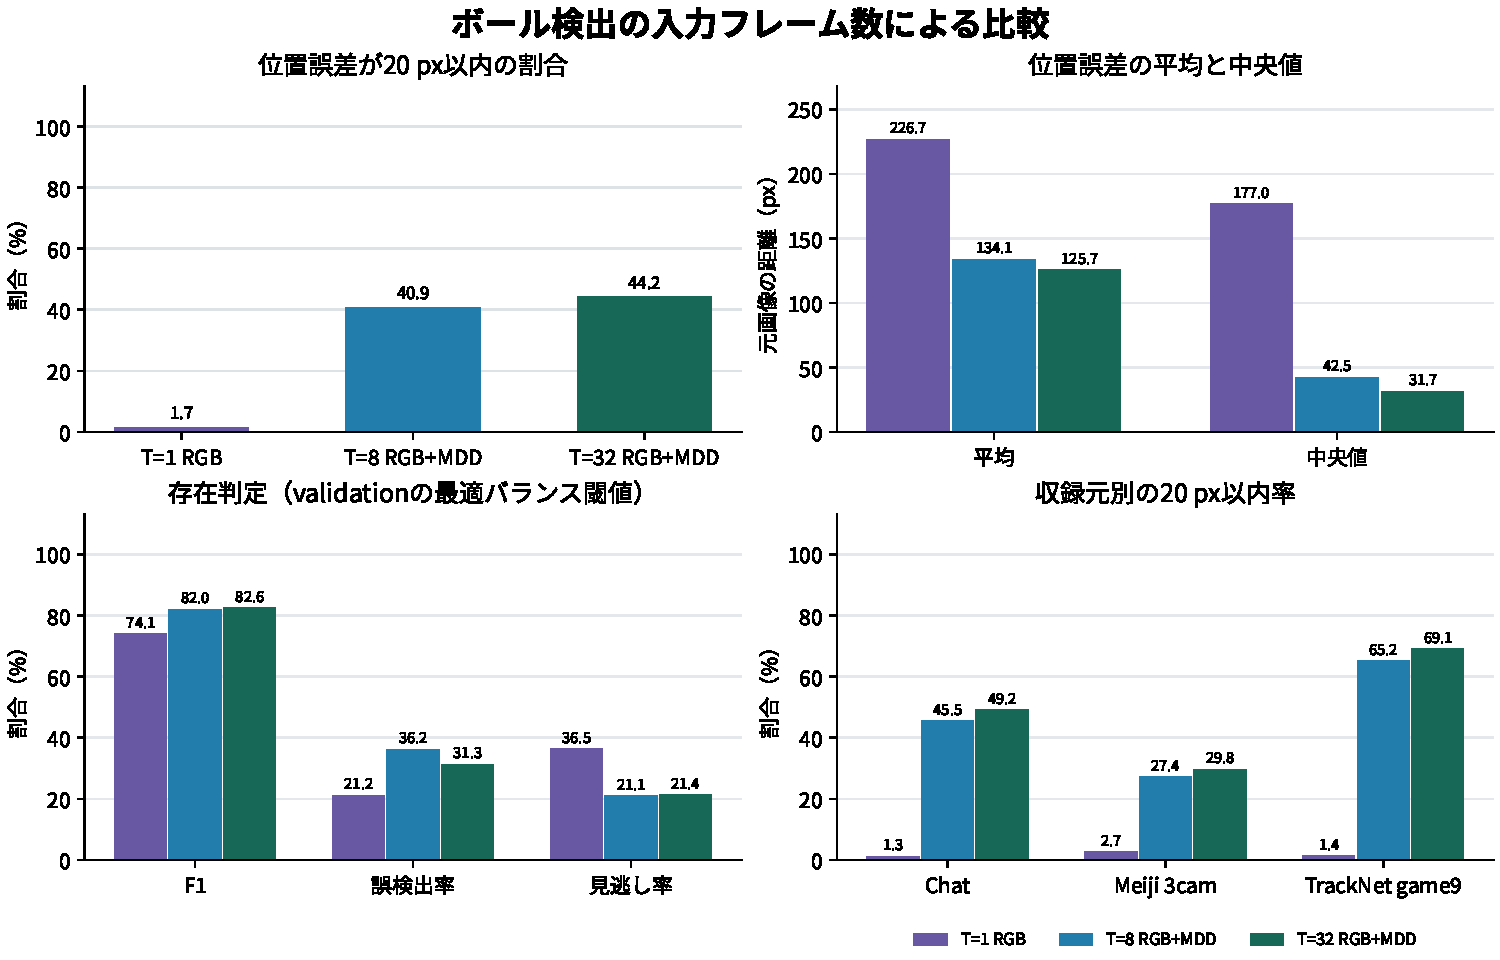
\includegraphics[width=\linewidth]{figures/ball/temporal_training_ablation.pdf}
\caption{同一学習予算での全validationの比較。位置は元画像px、存在F1は全validationで選んだ閾値を用いた。}
\label{fig:ball-training}
\end{figure}
\FloatBarrier

\section{実行システム}
\label{sec:execution-system}

\section{実験}
\label{sec:experiments}

\section{限界と今後の課題}
\label{sec:limitations}

\paragraph{コートの汎化と幾何教師}
学習規模を拡張して視点分布の広さと密度を独立に制御し、未知の収録で低角・横向き・見切れ別に採点する。
合成データの投影教師にはSfMの時間依存の誤差と地面の凹凸が入る。再訪時の幾何整合と独立の地面基準から両者を調べる。
実写の固定カメラでも、振動・ズーム・レンズ歪みや同期の残差は三角測量に伝わる。

\paragraph{IDと絶対3D精度}
停止クリップの介入では、修正したboxからのpose・外観の再抽出と、人物対応通過後の全時系列のID採点が残る。
少数の選手から作った疑似参照は、採点に使った観測と由来が重なる。全画面の人物検出の適合率は未集計である。
独立参照に対する球位置・選手関節・rootの絶対3D誤差は未計測である。
モーションキャプチャや独立に校正した観測を同じ時刻とコート座標に揃え、IDの一致、位置誤差、欠測を同時に測る。

\paragraph{球像と時系列}
初版の外部注釈は生成モデルと実行IDが未確認である。
母集団の画面外率と遮蔽率を測るには、層化した目視例に加え、蓄積した推定座標を照合する独立の参照が要る。
単フレームと時系列の差にはMDDの寄与が含まれる。時間長の寄与を調べるには、入力特徴を揃えた比較を複数seedと独立testに広げる。

\paragraph{実行系の測定範囲}
横断バッチの効果を測るには、クリップ規模、形状分布、保存済み成果物、OSのキャッシュ状態を揃えた反復計測が要る。
横断バッチを外したTensorRT構成の計時が残る。実行条件間の出力差は、座標差の最大値と有効性マスクの変化も追う。

\section{おわりに}
\label{sec:conclusion}

同期固定カメラからテニスのプレイヤーとボールを同じコート座標に復元する標準経路を示した。
規格コートで視点を整列し、選手を対応付けて関節と球を三角測量する。身体姿勢、位置、球軌道を元動画の時間軸で統合し、
復元の有効性と失敗理由を保存する。
コートの学習シーン構成、選手選別、球検出の時間文脈を比較し、下流の観測を左右する要因を示した。
宣言型計画と成果物保存でラリー単位の処理を動画全体へ展開し、モデル共有とTensorRTによる
時間・資源の変化を、欠測と座標差の実測とともに報告した。


% 最初の引用を追加するときに次の二行を有効にする。
% \bibliographystyle{unsrt}
% \bibliography{references}

\clearpage
\appendix
\section{再現手順と追加資料}
\label{app:reproducibility}

\subsection{入力と公開サンプル}

再構成を追試するときは、カメラID・同期・解像度・FPS・元フレーム数をmanifestで固定する。
公開サンプルは \href{https://huggingface.co/datasets/Motoki098/tennis-lab-multiview-sample}{テニス多視点サンプル}
から取得し、リポジトリのデータroot基準で動画パスを指定する。
指定したモデル重み、外部ライブラリ、DINOの拡張、身体モデル資産を先に解決する。
配布版の再現と当時のv2保存については、
\href{https://github.com/Motoki0705/tennis-lab/blob/main/knowledge/nodes/tennis_scene/000028-run-multiview-sample-standard-pipeline-20261021.md}{公開サンプルの実行記録}
に固定入力のハッシュと実行版がある。

標準入口では公開シーンの版に合わせてイベント方式を明示する。GPU実行はリポジトリの共有キューを用いる。

\begin{verbatim}
.venv/bin/python -m src.tennis_scene.scripts.run_pipeline \
  'video_paths=[samples/cam0.mp4,samples/cam1.mp4,samples/cam2.mp4]' \
  'camera_ids=[cam0,cam1,cam2]' event_detection.method=rule
\end{verbatim}

一括入口は \texttt{run\_video\_batch} で、登録済み動画のID、dataset、pipeline設定と上書き設定を渡す。
固定コートを使う実験は共有成果物のdigestを指定し、プレイヤーのみの設定はそれをrunの入力記録へ保存する。
比較では条件ごとに空のstoreを用意し、出力を読む際は採用した依存鎖と配列のchecksumを照合する。

\subsection{SceneResult v2のマスクと理由コード}

表\ref{tab:scene-masks}に、標準経路が保存する再構成用のブールマスクを示す。
$P$は選手数、$T$は元フレーム数である。理由コード配列の型と形状は表\ref{tab:scene-contract}の注に従い、
値\ev{schema}{0}がマスクの真と一致する。
球の画像座標の利用可否は、視点別のブール配列 \texttt{ball\_vis} に保存する。

\begin{table}[htbp]
\centering
\caption{SceneResult v2の再構成マスク。理由欄は対応する保存配列の識別子。}
\label{tab:scene-masks}
\small
\begin{tabular}{@{}llll@{}}
\toprule
マスク & 形状 & 真の意味 & 理由コード配列 \\
\midrule
\texttt{player\_observed} & $(P,T)$ & 確定IDで実観測あり & --- \\
\texttt{player\_valid} & $(P,T)$ & SMPL rootの配置が有効 & \texttt{player\_rejection\_code} \\
\texttt{player\_heading\_valid} & $(P,T)$ & 身体のyawが有効 & --- \\
\texttt{player\_kp\_3d\_vis} & $(P,T,\ev{schema}{17})$ & 三角測量した関節が有効 & \texttt{player\_kp\_3d\_rejection\_code} \\
\texttt{player\_smpl\_valid} & $(P,T)$ & 身体メッシュの配置が有効 & --- \\
\texttt{ball\_3d\_valid} & $(T,)$ & 球の三角測量が有効 & \texttt{ball\_rejection\_code} \\
\bottomrule
\end{tabular}
\end{table}

表\ref{tab:scene-reasons}のroot・関節・球は、それぞれ表\ref{tab:scene-masks}の
選手root・三角測量関節・球に対応する理由コード配列を指す。
関節または球の復元出力がない場合と、モデルによる球の有効フレーム数が設定下限に届かない場合は、
対応する理由コード配列を値\ev{point-rejections}{1}で満たす。
外部注釈から球を復元する設定では、利用可能な視点が足りない場合は値\ev{point-rejections}{1}、
視点が足りていても幾何が成立しない場合は値\ev{point-rejections}{7}を使う。

\begin{table}[htbp]
\centering
\caption{再構成で保存する非ゼロの理由コード。}
\label{tab:scene-reasons}
\small
\begin{tabular}{@{}rllp{.53\linewidth}@{}}
\toprule
値 & 対象 & 実装名 & 意味 \\
\midrule
\ev{player-rejections}{1} & root & --- & 身体復元または身体配置の出力がない。 \\
\ev{point-rejections}{1} & 関節・球 & \texttt{INSUFFICIENT\_VIEWS} & 利用できる視点が不足した。 \\
\ev{point-rejections}{2} & 関節・球 & \texttt{DEGENERATE\_RAYS} & 視線がほぼ平行か、線形初期解が得られなかった。 \\
\ev{point-rejections}{3} & 関節・球 & \texttt{BEHIND\_CAMERA} & カメラ前方の解が得られなかった。 \\
\ev{point-rejections}{4} & 関節・球 & \texttt{REPROJECTION} & 再投影誤差が許容範囲に収まらなかった。 \\
\ev{point-rejections}{5} & 関節・球 & \texttt{OUTSIDE\_BOUNDS} & 水平位置または高さがコート座標の許容範囲外。 \\
\ev{point-rejections}{6} & root・球 & \texttt{EXCESSIVE\_SPEED} & 過大速度となる隣接フレーム対の両端を棄却した。 \\
\ev{point-rejections}{7} & 関節・球 & \texttt{OPTIMIZATION\_FAILED} & 三角測量の最適化の失敗または非有限解。 \\
\ev{player-rejections}{101} & root & \texttt{INSUFFICIENT\_JOINTS} & 配置に使える関節の数が不足した。 \\
\ev{player-rejections}{102} & root & \texttt{UNOBSERVABLE\_YAW} & 初期yaw補正を求める水平面での幾何支持が不足。 \\
\ev{player-rejections}{103} & root & \texttt{INSUFFICIENT\_SCALE} & スケール推定に使える対応骨長の組が不足した。 \\
\ev{player-rejections}{104} & root & \texttt{SCALE\_OUT\_OF\_RANGE} & 推定した選手のスケールが設定範囲を外れた。 \\
\ev{player-rejections}{105} & root & \texttt{SOLVER\_FAILED} & 区間の時系列配置の最適化の失敗または非有限解。 \\
\bottomrule
\end{tabular}
\end{table}

\subsection{採点単位と証拠の追跡}

採点単位と母数は各実験の表に従う。共通有効集合で精度を比べる場合は、共通集合へ含めた点と除外した点を記録する。
時間とメモリの計測では計測範囲、同期設定、プロセス数を固定し、モデル読込と推論の区間を分ける。

\subsection{図表の再生成と照合}

原稿ディレクトリの \texttt{evidence/claims.md} に、本文・表・図の指標、評価条件、対応する保存データと版を記した。
\texttt{evidence/figures.md} に元図の再現手順、コピー元と掲載先、SHA-256を記した。
固定資料のGitオブジェクトを取得する手順は原稿ディレクトリのREADMEにある。
次のコマンドはリポジトリのルートで実行する。追跡チェック付きの組版にはLaTeX入力のGit登録が必要である。

\begin{verbatim}
paper=paper/tennis_scene_architecture
.venv/bin/python -B "$paper/scripts/make_tables.py"
.venv/bin/python -B "$paper/scripts/prepare_figures.py" --restore
bash "$paper/scripts/make_diagrams.sh"

.venv/bin/python -B "$paper/scripts/make_tables.py" --check
.venv/bin/python -B "$paper/scripts/prepare_figures.py"
.venv/bin/python -B "$paper/scripts/check_evidence.py"
bash "$paper/build.sh" --check-tracked
\end{verbatim}


\end{document}
